%!TEX root = bachelor.tex
\chapter{Analyse}
analyse?

projektionsfehler bei dem einen
anzahl löcher bei dem anderen

prjektionsfehler ohne kalib ist wesentlich größer, da die implizitie intrinsiche kalib durch die svd keine verzerrung entfernt

kann man untersucne wie sich die intrinsische kalibrierung auswirkt?

datenerhebung oder so was? laufzeit?

robustheit ransac ellipse?

robustheit reverse warping? bestimmung der keypoints?

laufzeitdurchschnitt pro bild  auf raspberry von 1000 bildern bei verschiedenen auflösungen

Raspberry Pi 2 Model B:
\begin{itemize}
	\item 900MHz ARM Cortex-A7 CPU
	\item 1GB RAM
	\item GCC-4.??? Release
	\item Opencv???, Qt????
\end{itemize}


\begin{figure}[!htb]
	\centering
	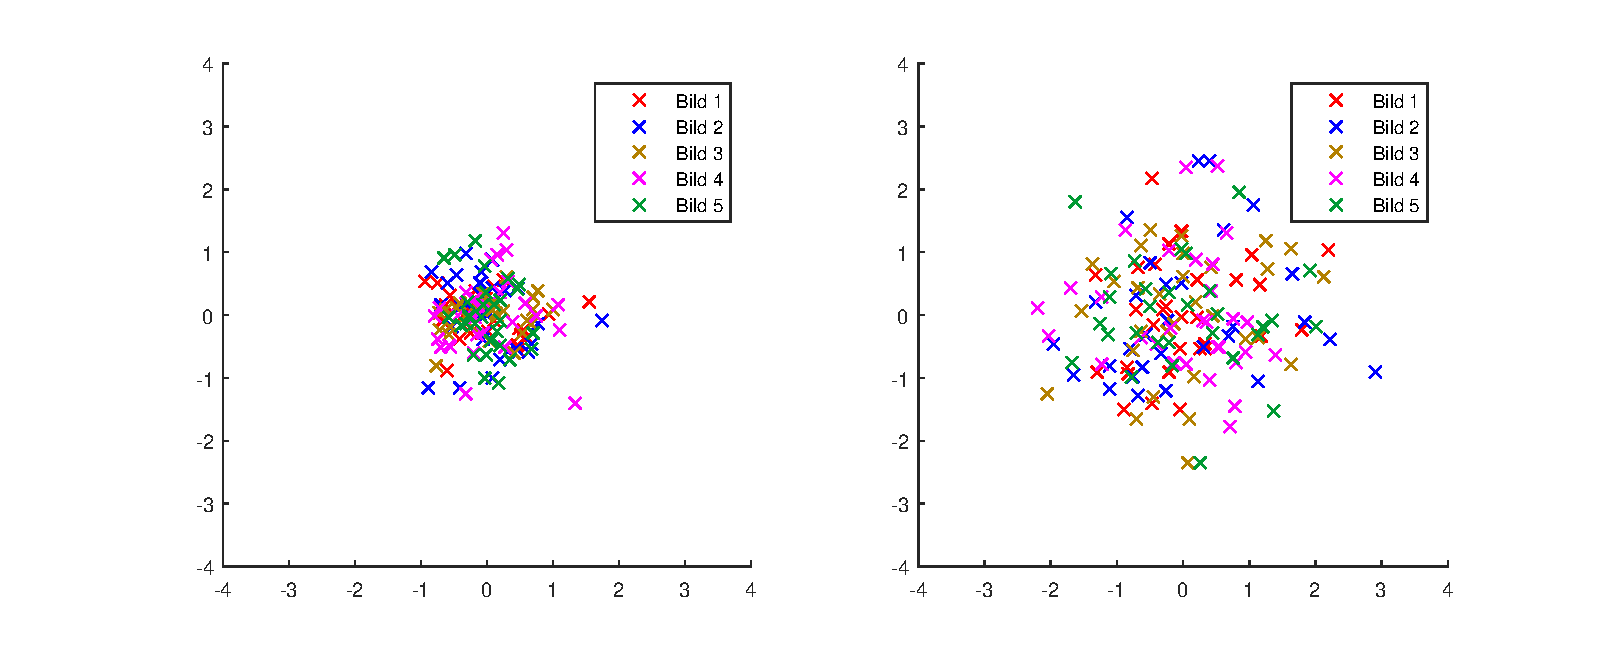
\includegraphics[width=\textwidth]{images/reprojectionErrorReverse.eps}
	\caption{Einfluss der intrinischen Kalibrierung}
	\label{fig:influenceCalib}
\end{figure}


\begin{figure}[!htb]
	\centering
	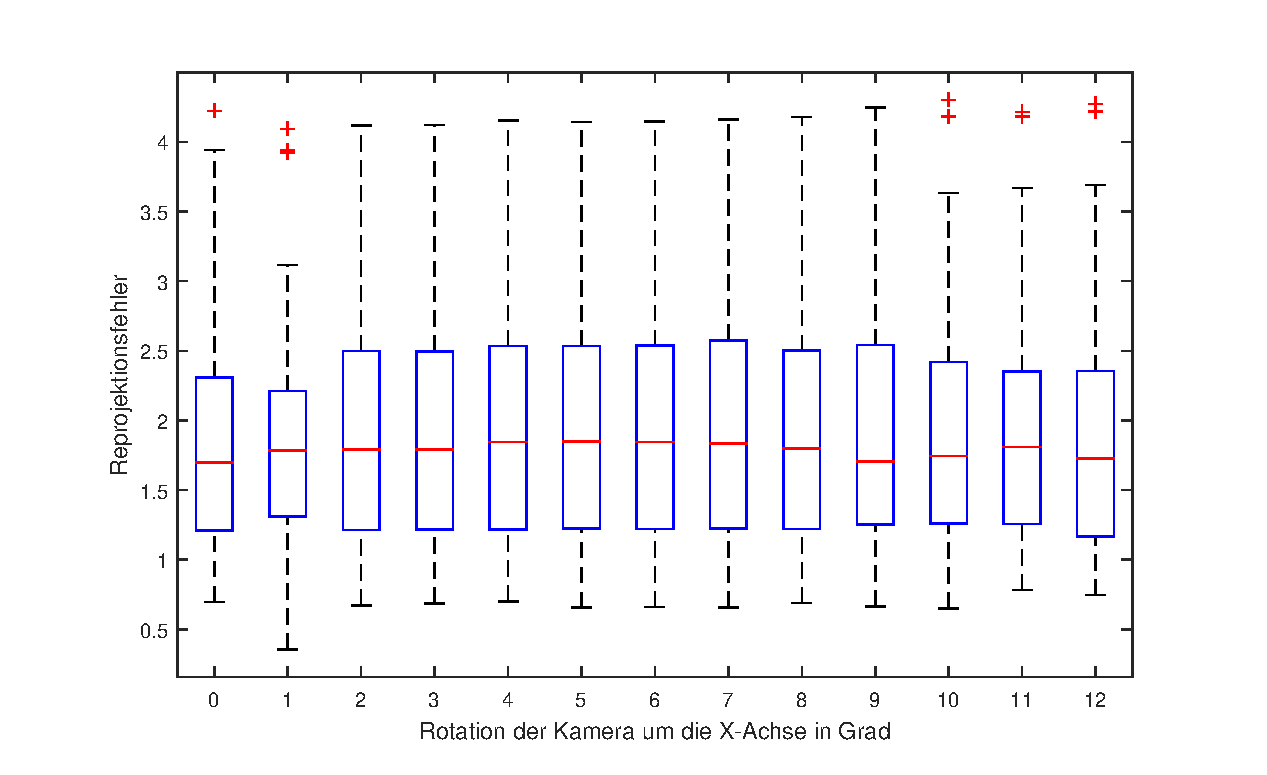
\includegraphics[width=\textwidth]{images/reprojectionErrorDeg.eps}
	\caption{Einfluss der Rotation der Kamera}
	\label{fig:influenceRot}
\end{figure}

\begin{figure}[!htb]
	\centering
	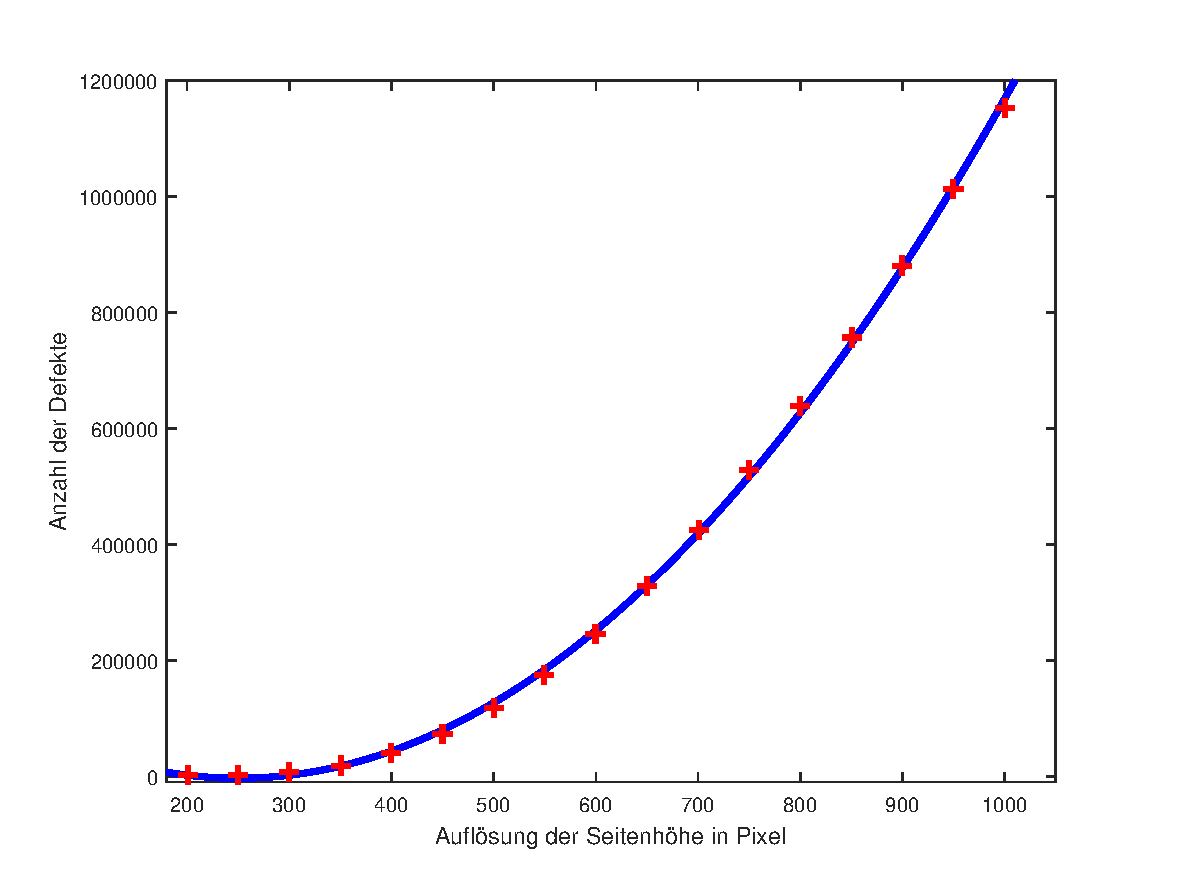
\includegraphics[width=\textwidth]{images/numberOfHoles.eps}
	\caption{Einfluss der intrinischen Kalibrierung}
	\label{fig:influenceRes}
\end{figure}


reprojection fehler unter verschiedenen Sichtwinkeln, Lichtverhältnissen?



\todo{LSQ irgendwo erklären}

\begin{figure}[!htb]
	\centering
	\begin{subfigure}{.5\textwidth}
		\centering
		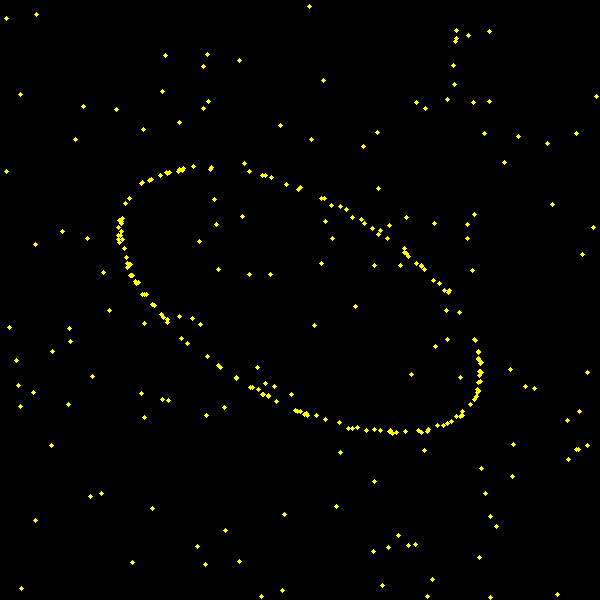
\includegraphics[width=.9\textwidth]{images/ransac50_0.png}
		\caption{gestörte Messdaten}
	\end{subfigure}%
	\begin{subfigure}{.5\textwidth}
		\centering
		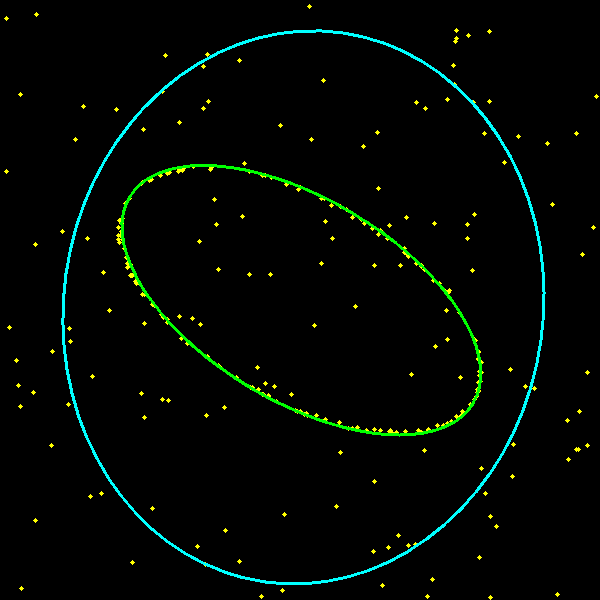
\includegraphics[width=.9\textwidth]{images/ransac50_1.png}
		\caption{detekt. Ellipsen: RANSAC (grün), LSQ (cyan)}
	\end{subfigure}
	\label{fig:bla}
	\caption{Vergleich RANSAC und LSQ bei gleichverteilten Ausreißern $\epsilon = 0.5, p = 0.99$}
\end{figure}

\begin{figure}[!htb]
	\begin{subfigure}{.5\textwidth}
		\centering
		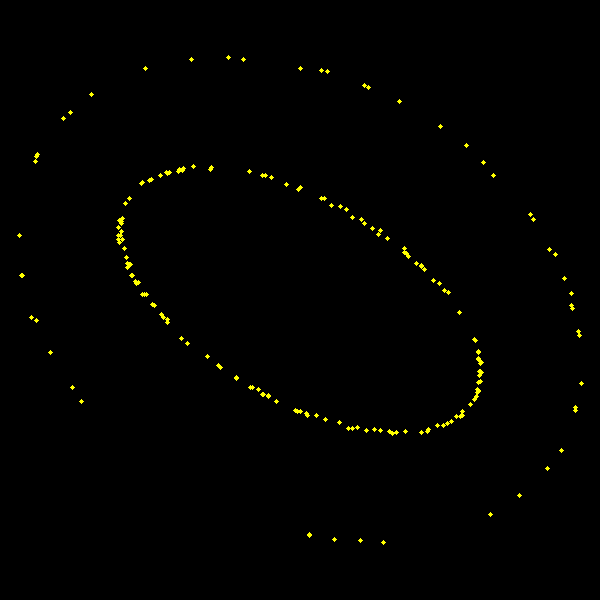
\includegraphics[width=.9\textwidth]{images/ransacShadow25_0.png}
	\end{subfigure}%
	\begin{subfigure}{.5\textwidth}
		\centering
		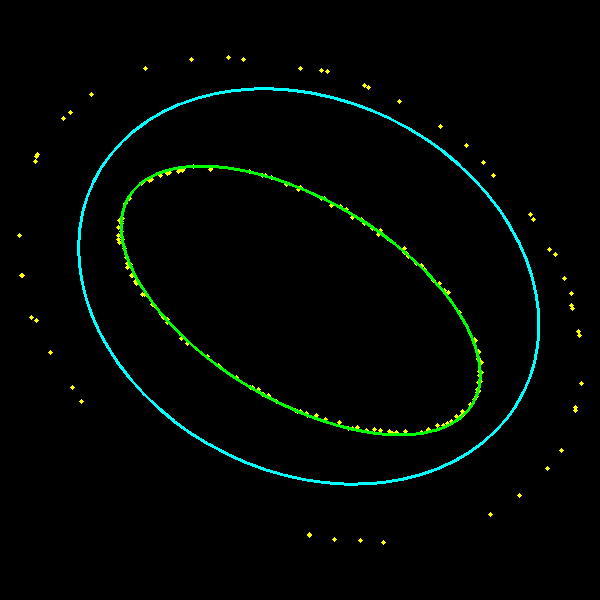
\includegraphics[width=.9\textwidth]{images/ransacShadow25_1.png}
	\end{subfigure}
	\begin{subfigure}{.5\textwidth}
		\centering
		\vspace{0.2cm}
		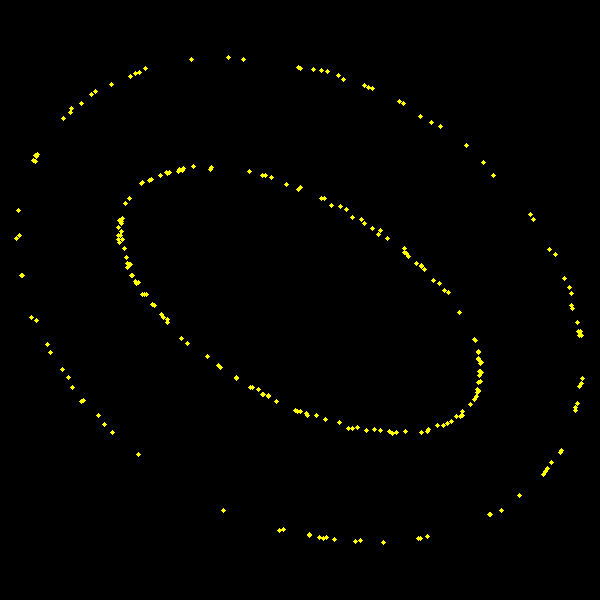
\includegraphics[width=.9\textwidth]{images/ransacShadow40_0.png}
	\end{subfigure}%
	\begin{subfigure}{.5\textwidth}
		\centering
		\vspace{0.2cm}
		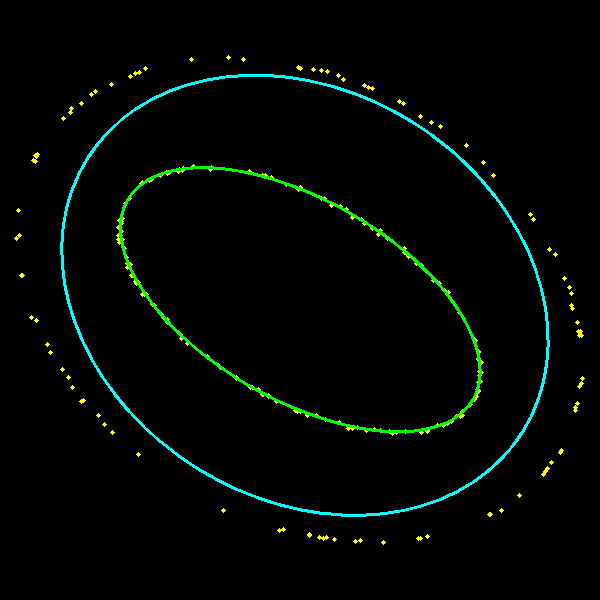
\includegraphics[width=.9\textwidth]{images/ransacShadow40_1.png}
	\end{subfigure}
	\caption{Vergleich RANSAC und LSQ bei Schattenellipsen mit $p = 0.99$ und $\epsilon = 0.25$ (oben), $\epsilon = 0.4$ unten, links gestörte Messdaten, rechts detektierte Ellipsen RANSAC (grün), LSQ (cyan)}
	\label{fig:blubb}
\end{figure}



\begin{figure}[!htb]
	\centering
	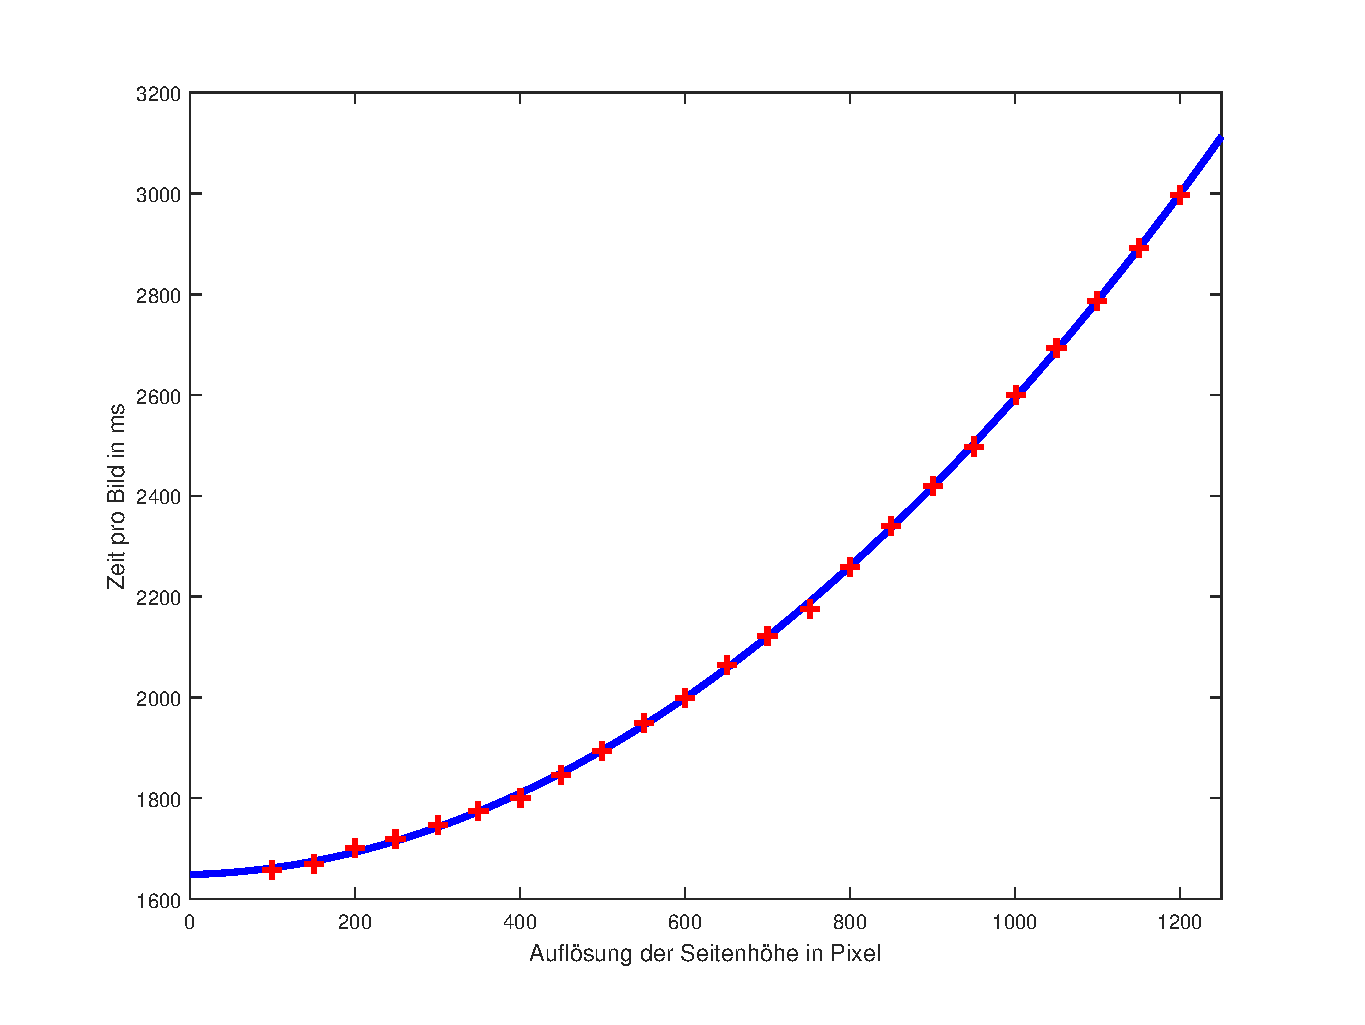
\includegraphics[width=\textwidth]{images/runningTimePerSlantheight.eps}
	\caption{Einfluss der intrinischen Kalibrierung}
	\label{fig:influenceRes}
\end{figure}
























